\subsection{EERD design}
\begin{figure}[H]
    \centering
    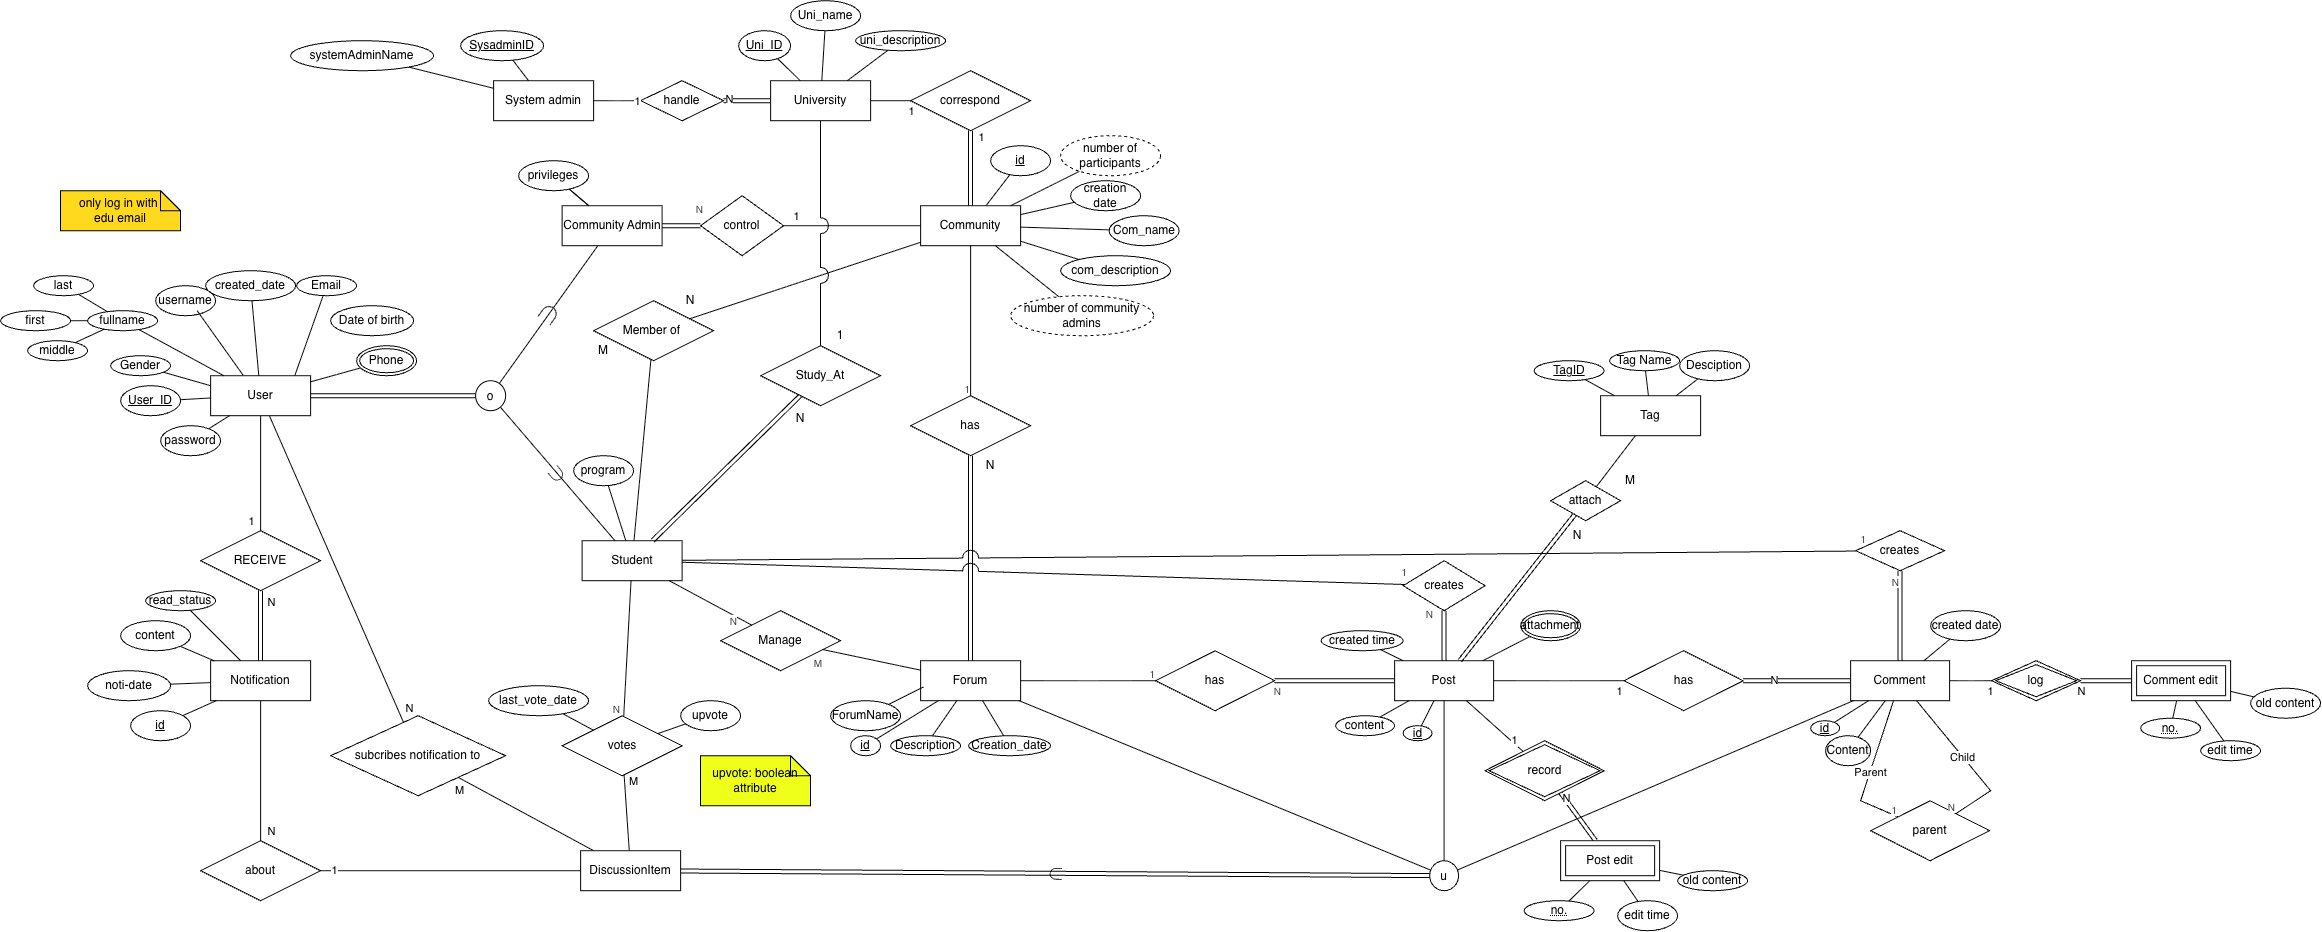
\includegraphics[width=1\textwidth]{Copy of erd.png}
    \caption{EERD model for StudentForum}
    \label{fig:eerd_model}
\end{figure}

Link for higher resolution: \href{https://drive.google.com/file/d/1kx8ZJ1E0M6ZHCK3iNVLn-PmnZDNYFnw0/view?usp=drive_link}{Team 4 eerd}

\subsubsection{Entity type and attributes}

The EERD consists of regular entity types, subtypes of \texttt{User}, a category
entity type, and two weak entity types. Their attributes are described below. There are 11 strong/regular entity types, 2 weak entity types, 1 category type. 
\noindent\textbf{USER (Regular entity):}
\begin{itemize}
    \item \texttt{User\_ID} (primary key)
    \item \texttt{Fullname} (composite attribute): \texttt{First}, \texttt{Middle}, \texttt{Last}
    \item \texttt{Username}
    \item \texttt{Password}
    \item \texttt{Email}
    \item \texttt{Phone} (multivalued attribute)
    \item \texttt{Gender}
    \item \texttt{Date of birth}
    \item \texttt{Created\_date}
\end{itemize}

\noindent\textbf{STUDENT (Subtype of USER):}
\begin{itemize}
    \item \texttt{Program}
\end{itemize}

\noindent\textbf{COMMUNITY ADMIN (Subtype of USER):}
\begin{itemize}
    \item \texttt{Privileges}
\end{itemize}

\noindent\textbf{SYSTEM ADMIN (Regular entity):}
\begin{itemize}
    \item \texttt{SysadminID} (primary key)
    \item \texttt{SystemAdminName}
\end{itemize}

\noindent\textbf{UNIVERSITY (Regular entity):}
\begin{itemize}
    \item \texttt{Uni\_ID} (primary key)
    \item \texttt{Uni\_name}
    \item \texttt{Uni\_description}
    \item \texttt{Email\_Domain}
\end{itemize}

\noindent\textbf{COMMUNITY (Regular entity):}
\begin{itemize}
    \item \texttt{ID} (primary key)
    \item \texttt{Com\_name}
    \item \texttt{Creation\_date}
    \item \texttt{Com\_description}
    \item \texttt{Number of participants} (derived attribute)
    \item \texttt{Number of community admins} (derived attribute)
\end{itemize}

\noindent\textbf{FORUM (Regular entity):}
\begin{itemize}
    \item \texttt{ID} (primary key)
    \item \texttt{ForumName}
    \item \texttt{Description}
    \item \texttt{Creation\_date}
\end{itemize}

\noindent\textbf{POST (Regular entity):}
\begin{itemize}
    \item \texttt{ID} (primary key)
    \item \texttt{Content}
    \item \texttt{Created time}
    \item \texttt{Attachment} (multivalued attribute)
\end{itemize}

\noindent\textbf{COMMENT (Regular entity):}
\begin{itemize}
    \item \texttt{ID} (primary key)
    \item \texttt{Content}
    \item \texttt{Created date}
\end{itemize}

\noindent\textbf{NOTIFICATION (Regular entity):}
\begin{itemize}
    \item \texttt{ID} (primary key)
    \item \texttt{Content}
    \item \texttt{Noti-date}
    \item \texttt{Read\_status}
\end{itemize}

\noindent\textbf{TAG (Regular entity):}
\begin{itemize}
    \item \texttt{TagID} (primary key)
    \item \texttt{Tag Name}
    \item \texttt{Description}
\end{itemize}

\noindent\textbf{DISCUSSION ITEM (Category entity type):}
\begin{itemize}
    \item This category is formed from \texttt{Forum}, \texttt{Post}, and \texttt{Comment}; it has no intrinsic attributes in the EERD.
\end{itemize}

\noindent\textbf{POST EDIT (Weak entity):}
\begin{itemize}
    \item \texttt{No.} (partial key)
    \item \texttt{Old content}
    \item \texttt{Edit time}
\end{itemize}

\noindent\textbf{COMMENT EDIT (Weak entity):}
\begin{itemize}
    \item \texttt{No.} (partial key)
    \item \texttt{Old content}
    \item \texttt{Edit time}
\end{itemize}

\subsubsection{Relations}

The EERD contains 19 relationships. The maximum cardinalities shown in the
diagram are described below.

\begin{itemize}
    \item \textbf{MEMBER OF:} \texttt{STUDENT} (M) -- \texttt{COMMUNITY} (N). A student may be a member of multiple communities, and a community may have multiple student members.

    \item \textbf{CONTROLS:} \texttt{COMMUNITY} (1) -- \texttt{COMMUNITY ADMIN} (N). A community can be controlled by multiple community administrators; each community administrator controls one community.

    \item \textbf{HAS (Community--Forum):} \texttt{COMMUNITY} (1) -- \texttt{FORUM} (N). A community can contain multiple forums, while each forum belongs to one community.

    \item \textbf{MANAGES:} \texttt{STUDENT} (N) -- \texttt{FORUM} (M). A student may manage multiple forums, and a forum may be managed by multiple students.

    \item \textbf{HAS (Forum--Post):} \texttt{FORUM} (1) -- \texttt{POST} (N). A forum can contain multiple posts, while each post belongs to one forum.

    \item \textbf{CREATES (Student--Post):} \texttt{STUDENT} (1) -- \texttt{POST} (N). A student can create multiple posts, while each post is created by one student.

    \item \textbf{HAS (Post--Comment):} \texttt{POST} (1) -- \texttt{COMMENT} (N). A post can have multiple comments, while each comment belongs to one post.

    \item \textbf{CREATES (Student--Comment):} \texttt{STUDENT} (1) -- \texttt{COMMENT} (N). A student can create multiple comments, while each comment is created by one student.

    \item \textbf{PARENT (recursive):} \texttt{COMMENT} (Parent: 1) -- \texttt{COMMENT} (Child: N). A parent comment can have multiple child comments, and each child comment has one parent comment.

    \item \textbf{ATTACHES:} \texttt{POST} (N) -- \texttt{TAG} (M). A post can be associated with multiple tags, and a tag can be attached to multiple posts.

    \item \textbf{VOTES:} \texttt{STUDENT} (N) -- \texttt{DISCUSSION ITEM} (M). A student can vote on multiple discussion items, and a discussion item can receive votes from multiple students. This relationship has the attributes \texttt{Upvote} (Boolean) and \texttt{Last\_vote\_date}.

    \item \textbf{SUBSCRIBES NOTIFICATION TO:} \texttt{USER} (N) -- \texttt{DISCUSSION ITEM} (M). A user can subscribe to notifications for multiple discussion items, and a discussion item can have multiple subscribing users.

    \item \textbf{RECEIVES:} \texttt{USER} (1) -- \texttt{NOTIFICATION} (N). A user can receive multiple notifications, while each notification is received by one user.

    \item \textbf{ABOUT:} \texttt{NOTIFICATION} (N) -- \texttt{DISCUSSION ITEM} (1). A discussion item can be the subject of multiple notifications, while each notification is about one discussion item.

    \item \textbf{STUDIES AT:} \texttt{STUDENT} (N) -- \texttt{UNIVERSITY} (1). A university can have multiple students, while each student studies at one university.

    \item \textbf{HANDLES:} \texttt{SYSTEM ADMIN} (1) -- \texttt{UNIVERSITY} (N). A system administrator can handle multiple universities, while each university is handled by one system administrator.

    \item \textbf{CORRESPONDS:} \texttt{UNIVERSITY} (1) -- \texttt{COMMUNITY} (1). Each university corresponds to one community, and each community corresponds to one university.

    \item \textbf{RECORDS (identifying):} \texttt{POST} (1) -- \texttt{POST EDIT} (N). A post can have multiple edit records; each \texttt{Post Edit} is identified through one post.

    \item \textbf{LOGS (identifying):} \texttt{COMMENT} (1) -- \texttt{COMMENT EDIT} (N). A comment can have multiple edit records; each \texttt{Comment Edit} is identified through one comment.
\end{itemize}

\noindent\textbf{Specialization and category constraints:}
\begin{itemize}
    \item \texttt{STUDENT} and \texttt{COMMUNITY ADMIN} are overlapping subtypes of \texttt{USER}, as indicated by the \texttt{o} specialization circle.
    \item \texttt{DISCUSSION ITEM} is a union/category formed from \texttt{FORUM}, \texttt{POST}, and \texttt{COMMENT}, as indicated by the \texttt{u} category circle.
\end{itemize}

